\section{Approach and Uniqueness\label{sec:approach}}
\begin{figure}
    \begin{center}
        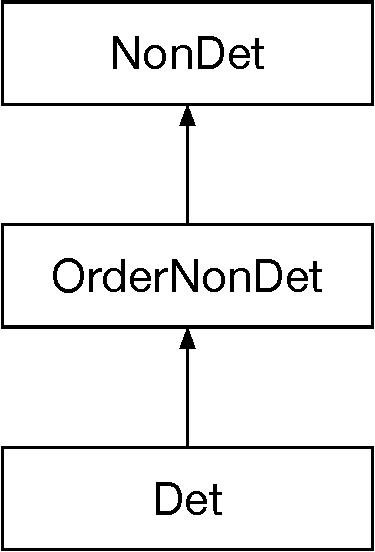
\includegraphics[scale=0.37]{detHierarchy}
    \end{center}
    \caption{Determinism type qualifier hierarchy}
    \label{fig:determinism-hierarchy}
\end{figure}

We solve the problem of detecting nondeterminism by introducing a type system
that allows programmers to express nondeterminism properties in a program that can be checked
at compile time.
The most novel part of our analysis is how it handles collections that will
contain the same values, but
possibly in a different order, on different runs.


%\todo{This is the first mention of
%    the determinism type system, and the first mention of types since the
%    abstract.  This is sudden and unexpected, and it will confuse readers.
%    You need to say that you will take this approach to solving the problem!}
%\todo{The introduction of the type
%    qualifiers is too sudden, too.  What are type qualifiers?  How are they
%    used?  Why does a reader care?  You should say that every expression in
%    the program is classified as one of the following categories.}

A type abstracts or restricts the set of possible
run-time values that an expression may evaluate to and the operations that may be performed.
A programming language provides \emph{basetypes}, such as \<Int>.
A \textit{type qualifier} on a basetype adds additional constraints;
that is, it reduces the size of the set of values.
An example type qualifier is \<Positive>, and a type (which combines a qualifier
and a basetype) is \<Positive Int>.
The core of the determinism type system
is the following type qualifiers:
\begin{itemize}
    \item \<NonDet> indicates
    that the expression might have different values in two different executions.
    \item \<OrderNonDet> indicates that the expression is a collection or
    a map that contains the same elements in every execution, but possibly
    in a different order.
    \item \<Det> indicates that the expression evaluates to equal values in
    all executions; for a collection, iteration
    also yields the values in the same order.
\end{itemize}
\Cref{fig:determinism-hierarchy} shows the subtyping
relationship among the qualifiers.
Programmers can write these type qualifiers to specify their program's behavior.

Every expression in a program is classified as either \<NonDet>, \<OrderNonDet>, or  \<Det>.
%\todo{Cut the following sentence, which uses jargon like ``basetype'' that
%  has not been defined, and therefore is offputting and confusing to readers.}
%The basetypes of their elements can be specified independently of the collection basetypes.
%\todo{For the following sentence, show an example, or give the typing rule,
%  or both.}
However, an element type qualifier must be a subtype of the collection type qualifier.
For instance, the type \codeid{OrderNonDet Set<@Det String>} is valid since \<Det> is a subtype of
\<OrderNonDet>. The type \codeid{OrderNonDet Set<@NonDet String>} is invalid because the element type
(\<NonDet>) is not a subtype of the collection type (\<OrderNonDet>).

%\OurTypeSystem checks all the standard typing rules\todo{``all the standard
%  typing rules'' is too glib.  It denigrates the reader by implying that
%  the reader ought to know this already, or that the paper is intended only
%  for a narrow audience with a specific technical background.  Make the
%  paper more welcoming.  Give a couple examples, and maybe even show source
%  code for them.}
%of an object-oriented programming language where the types have these
%additional type qualifiers.
%\todo{The following three things are the same.  Why are they listed as
%  different?  Also, their purpose is to reduce false positive warnings,
%  rather than to enable better reporting of true positives.  Also, try to
%  explain terms when you introduce them.  If you don't have space for that,
%  then ask yourself if this point is important enough to include in the paper.}

\subsubsection{Behavior of order-nondeterministic collections}\label{sec:ond-behavior}
A collection of type \<OrderNonDet> has special properties. We elaborate on these properties
with examples below:
%\todo{Like other parts of the document (and as noted by the referees), this
%  feels vague.  Make it more concrete, with examples or with specific explanation.}

\begin{enumerate}
    \item
    The individual elements retrieved from it have type \<NonDet>.  This
    affects access, iteration, searching, etc.
    \begin{verbatim}
@OrderNonDet HashSet<Det String> set; 
// The type of elem is NonDet String
String elem = set.iterator().next();
    \end{verbatim}
    \vspace{-0.4cm}
    \item
    Size-related operations return a deterministic result.  This affects
    queries of whether an iterator has more elements.
    \begin{verbatim}
@OrderNonDet HashSet<Det String> set; 
// The type of elem is Det String
String elem = set.size();
    \end{verbatim}
    \vspace{-0.4cm}
    \item
    If the collection is sorted, or its elements are placed in a collection
    that does sorting, the result is deterministic.
    \begin{verbatim}
@OrderNonDet ArrayList<Det String> lst; 
// The type of sortedList is 
// @Det ArrayList<Det String>
ArrayList<Det String> sortedList = 
lst.sort();
    \end{verbatim}
    \vspace{-0.4cm}
\end{enumerate}

%%  LocalWords:  NonDet OrderNonDet Det basetype offputting basetypes
